% ==============================================
% ELEMENTO: DESENVOLVIMENTO
% ==============================================
\section{Desenvolvimento}
\label{sec:desenvolvimento}

\begin{figure}[H]
    \centering
    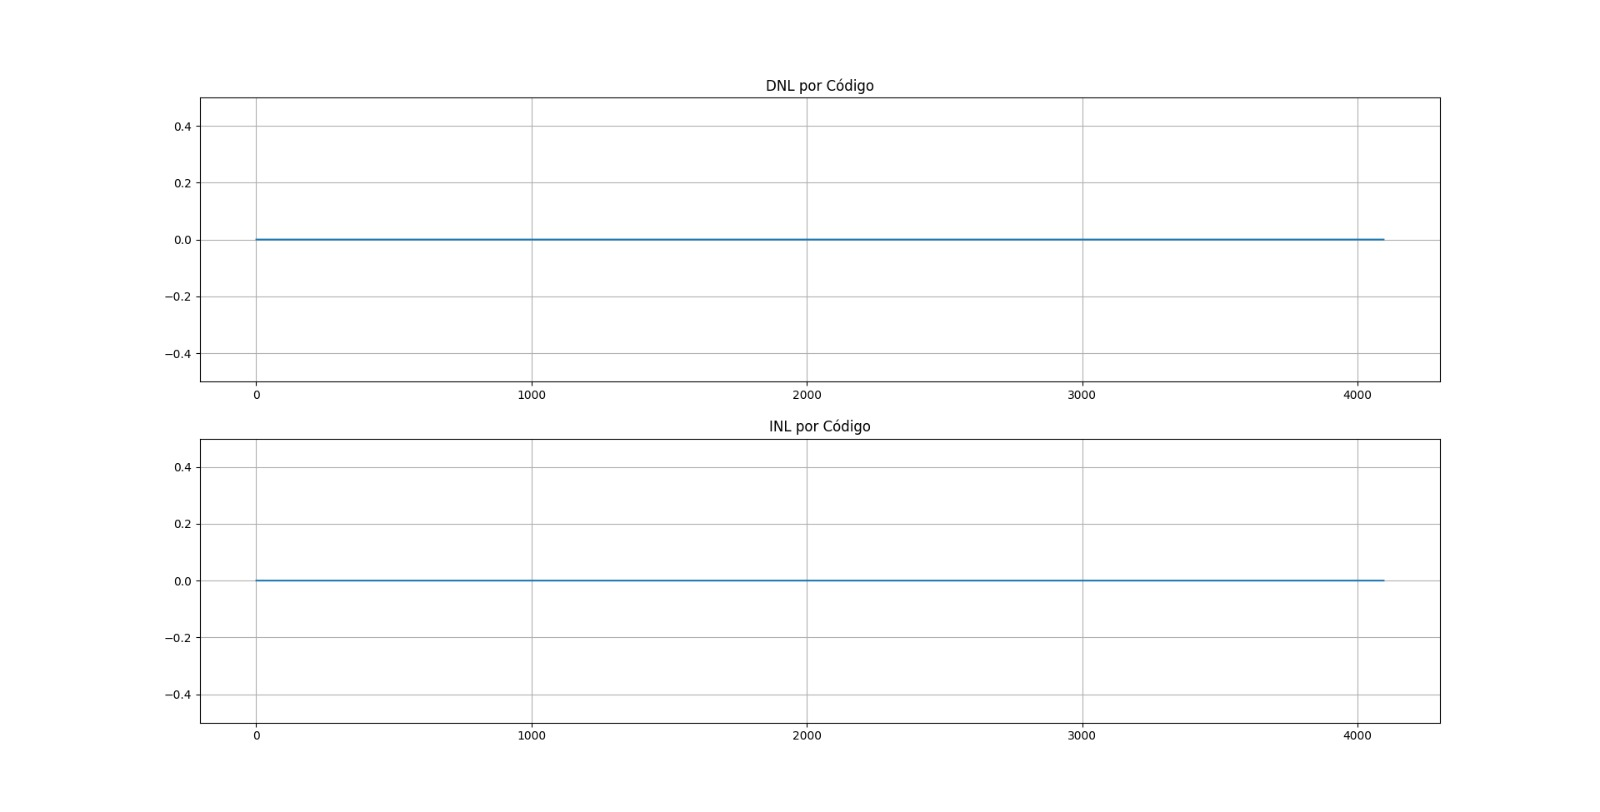
\includegraphics[width=0.8\textwidth]{IMAGENS/INL_DNL_0.jpg}
    \caption{INL e DNL.}
    \label{fig:inl_dnl_0}
\end{figure}

\begin{figure}[H]
    \centering
    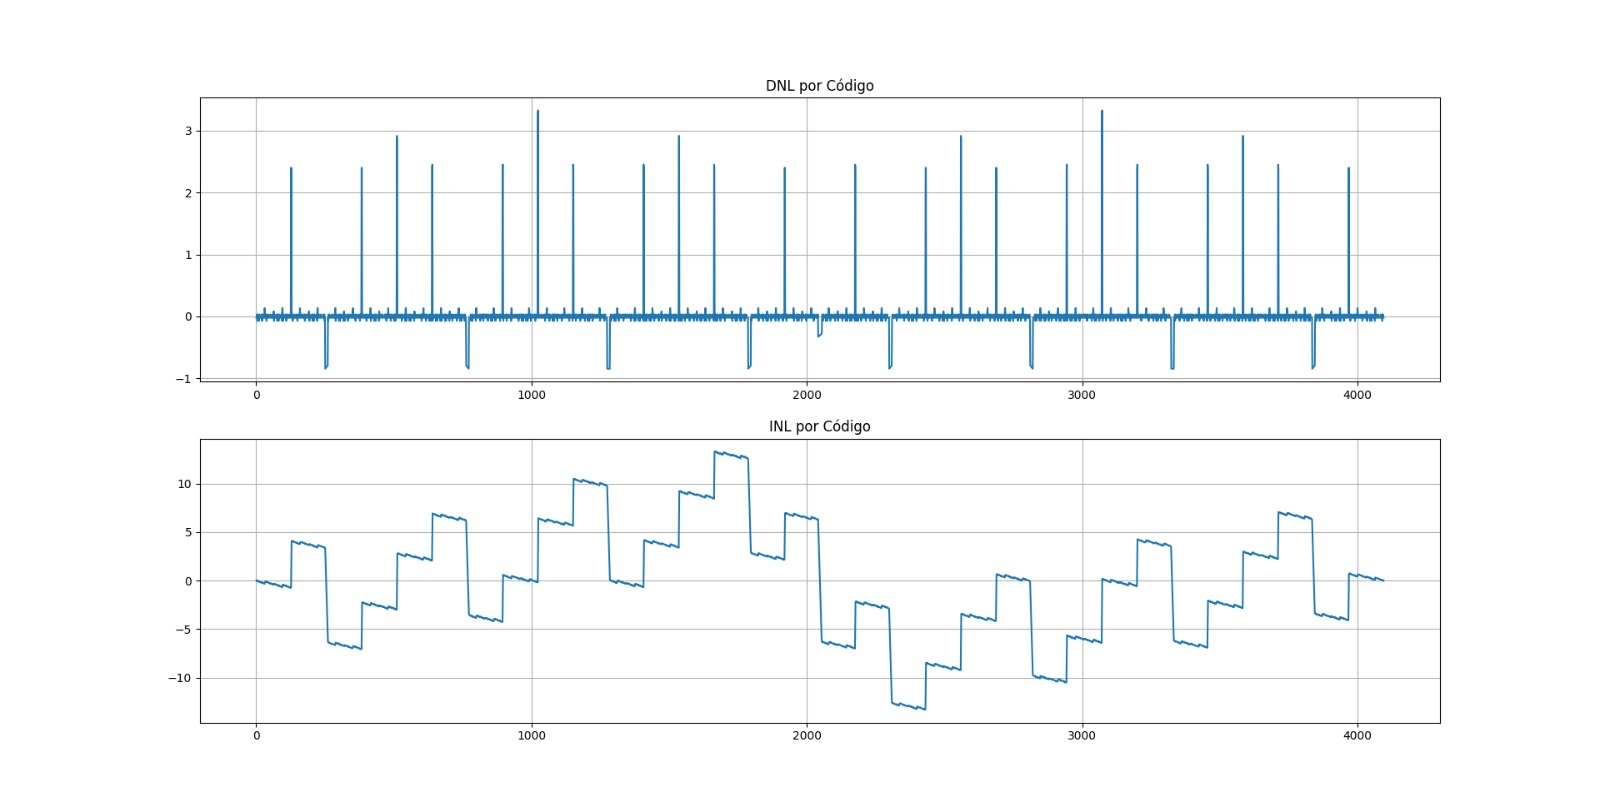
\includegraphics[width=0.8\textwidth]{IMAGENS/INL_DNL_codigo.jpg}
    \caption{INL e DNL do código.}
    \label{fig:inl_dnl_codigo}
\end{figure}

\begin{figure}[H]
    \centering
    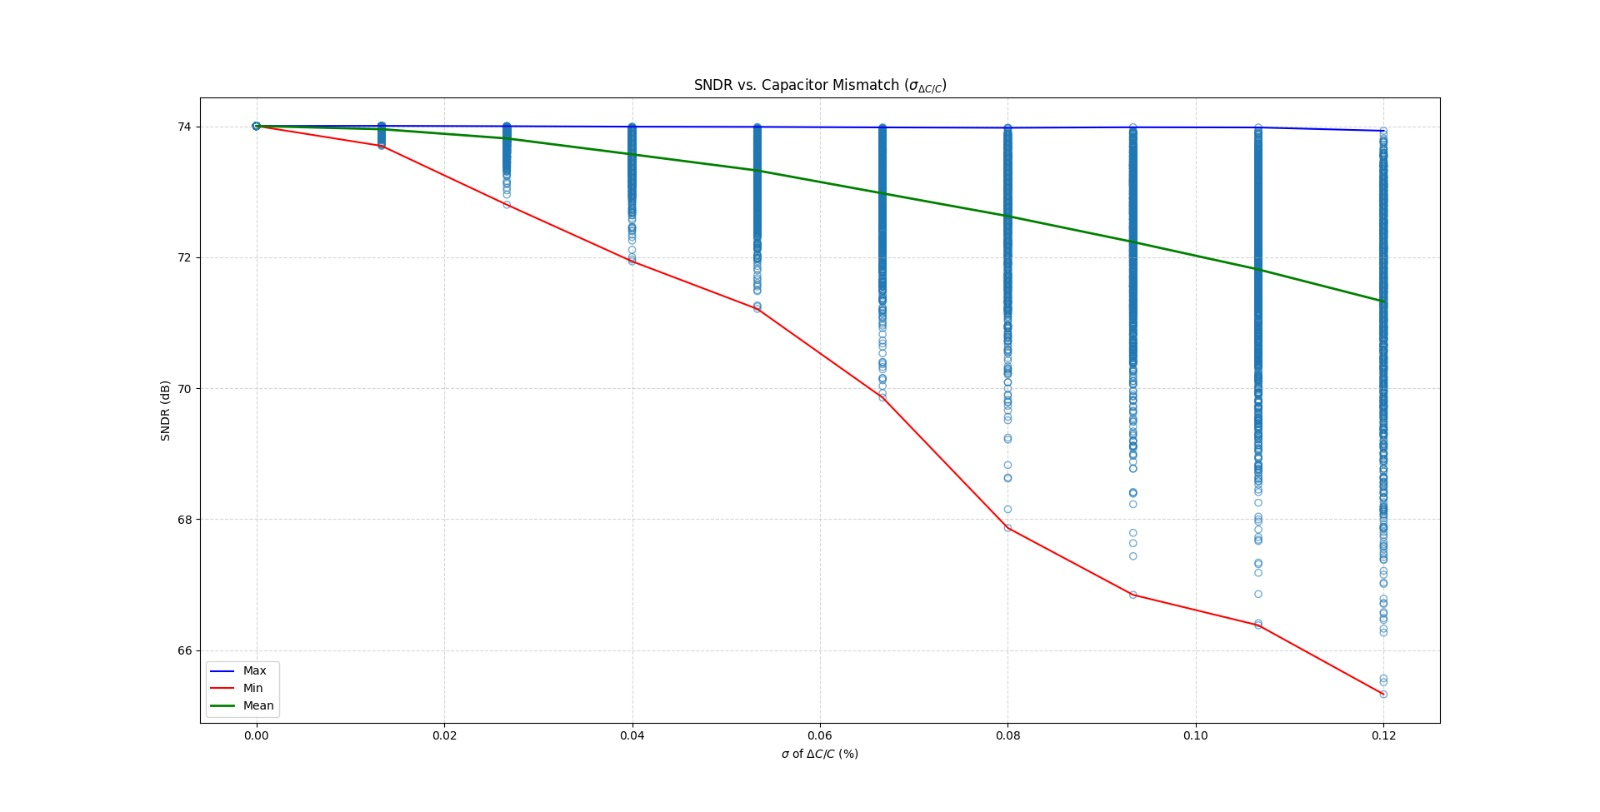
\includegraphics[width=0.8\textwidth]{IMAGENS/sndr_vs_mismatch.jpg}
    \caption{Mismatch entre os condensadores e influência na SNDR.}
    \label{fig:sndr_vs_mismatch}
\end{figure}

\begin{figure}[H]
    \centering
    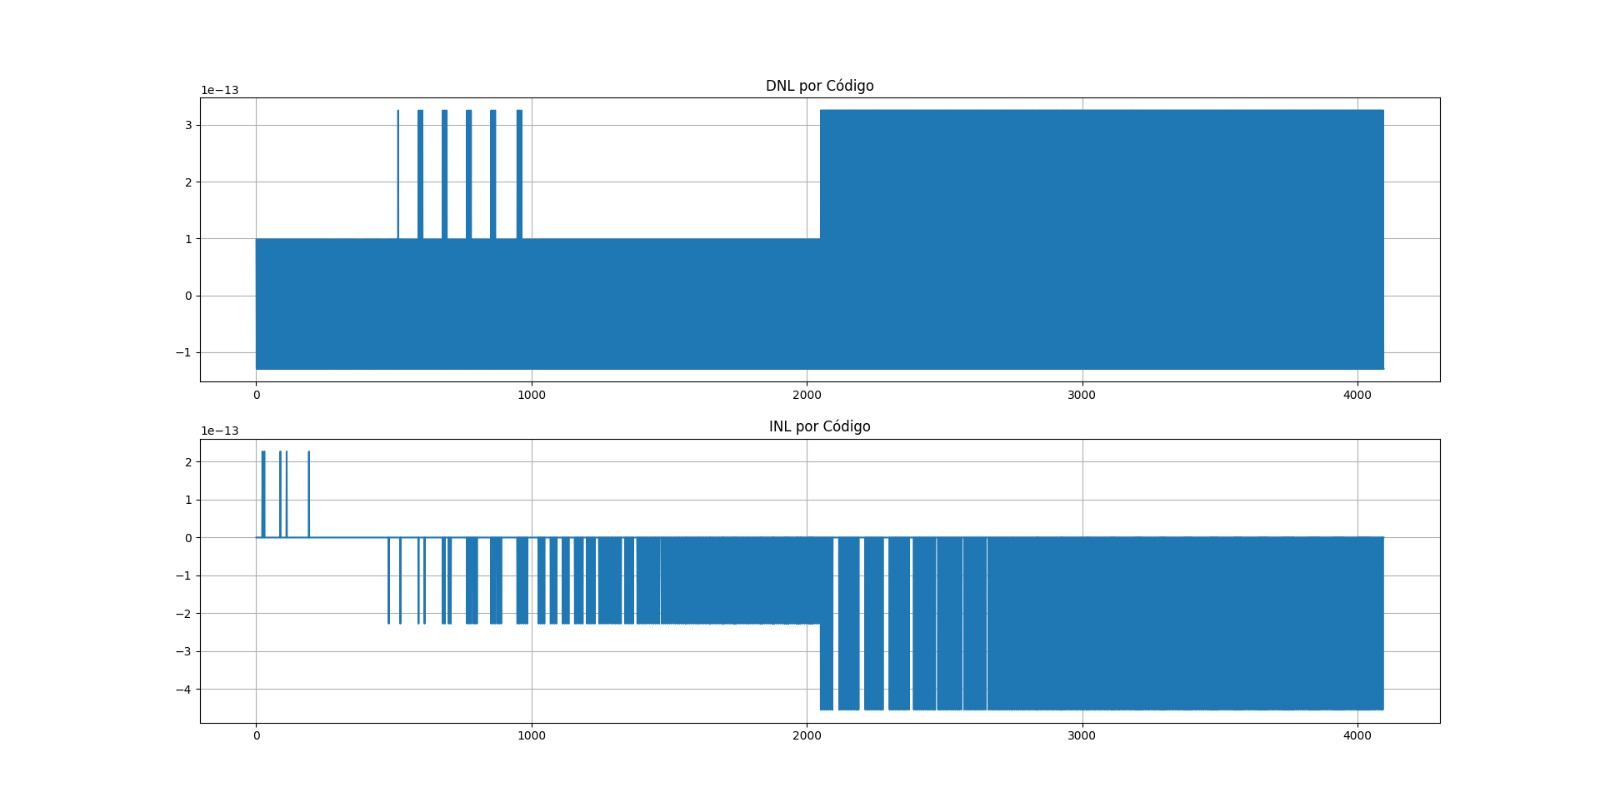
\includegraphics[width=0.8\textwidth]{IMAGENS/weird_INL_DNL.jpg}
    \caption{INL e DNL com erros.}
    \label{fig:weird_inl_dnl}
\end{figure}

\begin{figure}[H]
    \centering
    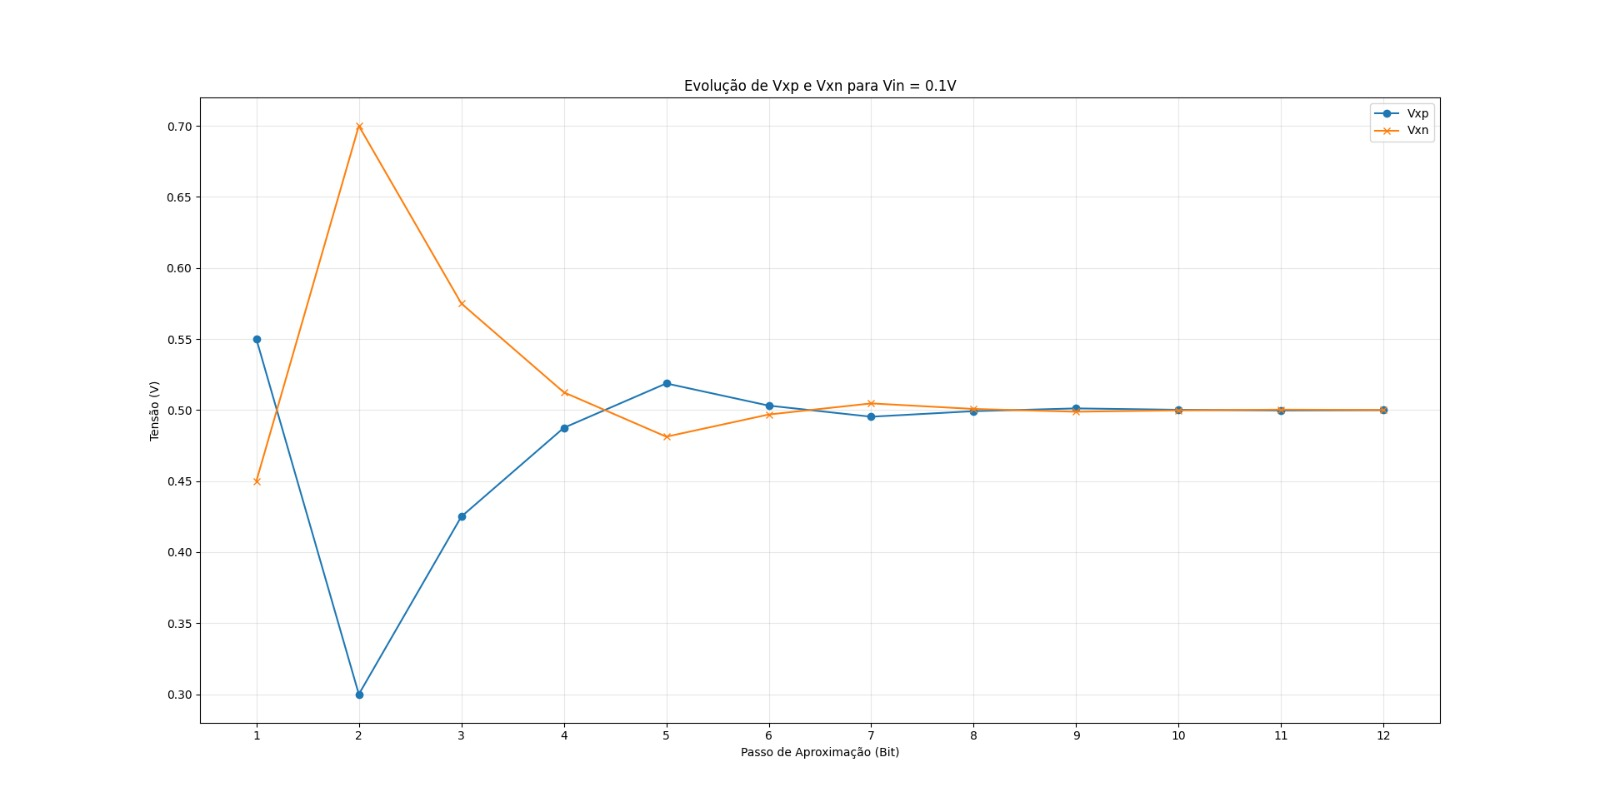
\includegraphics[width=0.8\textwidth]{IMAGENS/vxp_vs_vxn.jpg}
    \caption{Tensão do nó de sample positivo e comparaçao ao nó de sample negativo.}
    \label{fig:vxp_vs_vxn}
\end{figure}
